\nofiles
\documentclass[crop,tikz]{standalone}
\usepackage{amsmath}
\usepackage{amssymb}
\usepackage{tikz}
\usepackage{tikz-cd}

\usetikzlibrary{patterns, patterns.meta}
\begin{document}
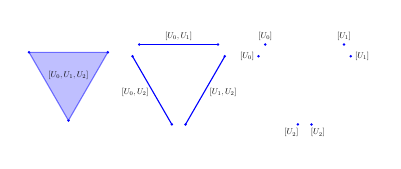
\begin{tikzpicture}
  \fill [fill=blue, opacity=1] (0,0) circle [radius=0.5pt];
  \fill [fill=blue, opacity=1] (1,0) circle [radius=0.5pt];
  \fill [fill=blue, opacity=1] ({1/2}, {-sqrt(3)/2}) circle [radius=0.5pt];

  \filldraw [thin, fill=blue!50, opacity=0.5, draw=blue] (0,0) -- (1,0) -- ({1/2}, {-sqrt(3)/2}) -- cycle;

  \node[scale=0.30] at ({1/2}, {-sqrt(3)/6}) {$[U_0, U_1, U_2]$};


  \fill [fill=blue, opacity=1] (1.4+0, 0+0.1) circle [radius=0.5pt];
  \fill [fill=blue, opacity=1] ({1.4+0-0.1*sin(60)}, {0-0.1*cos(60)}) circle [radius=0.5pt];
  \fill [fill=blue, opacity=1] (1.4+1, 0+0.1) circle [radius=0.5pt];
  \fill [fill=blue, opacity=1] ({1.4+1+0.1*sin(60)}, {0-0.1*cos(60)}) circle [radius=0.5pt];
  
  \fill [fill=blue, opacity=1] ({1.4+1/2-0.1*sin(60)}, {-sqrt(3)/2-0.1*cos(60)}) circle [radius=0.5pt];
  \fill [fill=blue, opacity=1] ({1.4+1/2+0.1*sin(60)}, {-sqrt(3)/2-0.1*cos(60)}) circle [radius=0.5pt];

  \draw [thin, draw=blue] (1.4+0, 0+0.1) -- (1.4+1, 0+0.1);
  \draw [thin, draw=blue] ({1.4+0-0.1*sin(60)}, {0-0.1*cos(60)}) -- ({1.4+1/2-0.1*sin(60)}, {-sqrt(3)/2-0.1*cos(60)});
  \draw [thin, draw=blue] ({1.4+1+0.1*sin(60)}, {0-0.1*cos(60)}) -- ({1.4+1/2+0.1*sin(60)}, {-sqrt(3)/2-0.1*cos(60)});

  \node[scale=0.30] at (1.4+1/2, 0+0.2) {$[U_0, U_1]$};
  \node[scale=0.30, anchor=west] at ({(1.4+1+1.4+1/2-0.1*sin(60))/2 + 0.15}, {(0+0.1-sqrt(3)/2-0.1*cos(60))/2-0.1}) {$[U_1, U_2]$};
  \node[scale=0.30, anchor=east] at ({(1.4+0+1.4+1/2-0.1*sin(60))/2 - 0.05}, {(0+0.1-sqrt(3)/2-0.1*cos(60))/2-0.1}) {$[U_0, U_2]$};

  \fill [fill=blue, opacity=1] (3.0+0, 0+0.1) circle [radius=0.5pt] node[scale=0.30, anchor=south, inner sep=5pt] {$[U_0]$};
  \fill [fill=blue, opacity=1] ({3.0+0-0.1*sin(60)}, {0-0.1*cos(60)}) circle [radius=0.5pt] node[scale=0.30, anchor=east, inner sep=5pt] {$[U_0]$};
  \fill [fill=blue, opacity=1] (3.0+1, 0+0.1) circle [radius=0.5pt] node[scale=0.30, anchor=south, inner sep=5pt] {$[U_1]$};
  \fill [fill=blue, opacity=1] ({3.0+1+0.1*sin(60)}, {0-0.1*cos(60)}) circle [radius=0.5pt] node[scale=0.30, anchor=west, inner sep=5pt] {$[U_1]$};
  
  \fill [fill=blue, opacity=1] ({3.0+1/2-0.1*sin(60)}, {-sqrt(3)/2-0.1*cos(60)}) circle [radius=0.5pt] node[scale=0.30, anchor=north, inner sep=5pt] {$[U_2]\quad\;\;$};
  \fill [fill=blue, opacity=1] ({3.0+1/2+0.1*sin(60)}, {-sqrt(3)/2-0.1*cos(60)}) circle [radius=0.5pt] node[scale=0.30, anchor=north, inner sep=5pt] {$\quad\;\; [U_2]$};
  

\end{tikzpicture}
\end{document}